
% POSTER EXAMPLE
%
% This is an example of a relatively sane poster. The box structure (and the
% narrative in general) is what I would expect, but it is completely
% non-mandatory; you may include whatever you want. Preferably, erase the
% existing box structure after you read it, and start from scratch.
%
% The main communication requirements for the poster that should be satisfied
% are as such:
%
% - At the defense, it should help you talk for around 10 minutes about your
%   thesis, and convince the committee that you did something interesting and
%   sufficiently complicated. Prepare pictures that explain your main results.
%
% - It should quickly communicate the main idea of your thesis to a random
%   educated by-walker. Ideally, a moderately-witted MFF graduate who has never
%   heard about your thesis before should be able to get the main "rough idea"
%   in less than 1 minute by just looking at the poster.

% modify the fontscale parameter to make everything slighly bigger or smaller.
% \documentclass[portrait,a0paper,fontscale=0.25]{baposter}
% \documentclass[portrait,a0paper,fontscale=0.26]{baposter}
% \documentclass[portrait,a0paper,fontscale=0.27]{baposter}
\documentclass[portrait,a0paper,fontscale=0.28]{baposter}

\usepackage[utf8]{inputenc}
\usepackage[T1]{fontenc}

% FONT CHOICES
% Posters do not need to be PDF/A; you can choose any relatable font from the
% TeX font catalogue without much risk. Sans-serif fonts are suggested for the
% posters; see https://tug.org/FontCatalogue/sansseriffonts.html
\usepackage[sfdefault]{Fira Sans}
%\usepackage[default]{droidsans}
%\usepackage[math]{iwona}
%\usepackage[defaultfam]{montserrat}
%\usepackage{cmbright}
%\usepackage{yfonts}\renewcommand{\familydefault}{\frakdefault}

\usepackage{color}
\usepackage{graphicx}
\usepackage{amssymb,amsmath}
\usepackage[export]{adjustbox} %allows using valign with \includegraphics

\renewcommand{\arraystretch}{1.5}

\usetikzlibrary{positioning}

% A WORD ABOUT COLORS
%
% This template is prepared with a relatively neutral gray background that
% gives decent box borders (with white and darker gray), does not clash with
% many colors (except for violet-brown and other mushroomish colors, perhaps)
% and gives a lot of space for highlighting stuff.
%
% Generally, other color variations are good too; there are no strict rules on
% the colors. Good choices include:
%
% - white backgrounds and differentiation of box headers by color (see
%   headerFontColor)
%
% - various slightly tinted backgrounds (try red!10 instead of black!3)
% 
% - dark backgrounds
%
% Keep in mind:
% - The normal "informative" text and figures should be DARK on LIGHT
%   background, not the other way around.
%
% - If you want a dark background, soften (darken) the box backgrounds a bit so
%   that they do not "shine" too much from the poster. Use \color{white} for
%   the heading, and switch the UK/MFF logos to white (see contents of logos/).
%
% - Do not mix too many color hues together. Most hues have their widely
%   accepted meaning (green: good result, red: problem, blue: information,
%   yellow: highlighter, brown: serious problem, violet: something really
%   weird/interesting/magic, depending on the shade).

% EXTRA PACKAGES AND DEFINITIONS I NEED

\usepackage{threeparttable} % for \tnote
\usepackage{hyperref} % for links
\usepackage{qrcode} % for qrcode
\usepackage{fontawesome} % for \faGithub
% https://github.com/EagleoutIce/fancyqr
\usepackage{fancyqr} % for fancy qrcode
\usepackage{bm} % boldface symbols (\bm)
\usepackage{booktabs} % for toprule, midrule etc.
\usepackage{xcolor} % for my custom colors

% Define the same colors as in my plots
% https://www.overleaf.com/learn/latex/Using_colors_in_LaTeX#Creating_your_own_colors
\definecolor{myblue}{RGB}{68, 117, 177}
\definecolor{myorange}{RGB}{207, 134, 59}
\definecolor{mygreen}{RGB}{89, 144, 65}
\definecolor{myred}{RGB}{172, 72, 66}

\begin{document}

\color{black!80} % default font color
\begin{poster}{grid=false,
	eyecatcher=true,
	background=plain,
	bgColorOne=black!3, % background color
	columns=2,
	headerborder=none,
	textborder=none,
	headershape=rectangle,
	headershade=plain,
	boxshade=plain,
	boxColorOne=white,
	headershade=plain,
	headerColorOne=black!15, % box header background color
	headerFontColor=black,
	}%
	{
\includegraphics[height=7em]{logos/mff-black.pdf}}
	{\vspace{-0.5ex} Traffic Signal Optimization}
	{\vspace{1ex} {\LARGE David Ruda} \\ Supervisor: RNDr. Jiří Fink, Ph.D. \\ \vspace{0.5ex} 2025}
	{
\includegraphics[height=7em]{logos/uk-red.pdf}}


%
% LEFT COLUMN
%

\begin{posterbox}[column=0,name=background]
{Problem}
% Describe what is the problem that your thesis addresses.
Traffic congestion is a growing issue in cities. Optimizing traffic signals is a cost-effective way to reduce delays and emissions without changing the physical infrastructure. The Google Hash Code 2021 competition introduced a simplified version of this real-world problem: \\

\textit{Given a city plan describing \textbf{intersections}, \textbf{streets}, and \textbf{cars} with planned paths through the city, optimize \textbf{\mbox{traffic light schedules}} to
maximize the number of cars reaching their destination before the deadline, while minimizing the overall time spent in traffic.}

\begin{center}
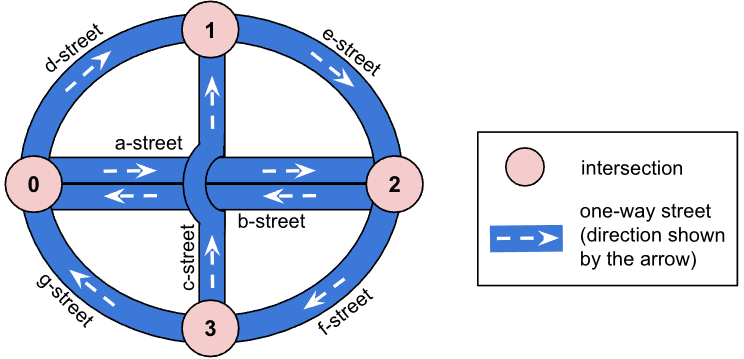
\includegraphics[width=1.0\linewidth]{img/figure1.png}
\small{Example of a city plan {[Google Hash Code 2021]}.}
\end{center}
\end{posterbox}

\begin{posterbox}[column=0, name=goals, below=background, headerColorOne=cyan!60, boxColorOne=cyan!20]{Thesis goals}
\begin{itemize}
\item Implement a \textbf{fast and efficient C++ simulator} for the problem and wrap it as a \textbf{Python package} for convenient use
\item Integrate the simulator into an optimization pipeline with three heuristic algorithms: \textbf{Genetic Algorithm}, \textbf{Hill Climbing}, and \textbf{Simulated Annealing}
\item Compare the performance of these algorithms on provided competition datasets
\end{itemize}

% Highlighting important boxes helps a lot, but do not overdo the highlighting --- if all boxes are highlighted, not a single one will actually stand out.
\end{posterbox}

\begin{posterbox}[column=0, name=something1, below=goals]{Traffic Light Schedule for one Intersection}
Each incoming street has two parameters: the \textbf{order} in which it gets a green light, and the \textbf{duration} of the green light.
\begin{center}
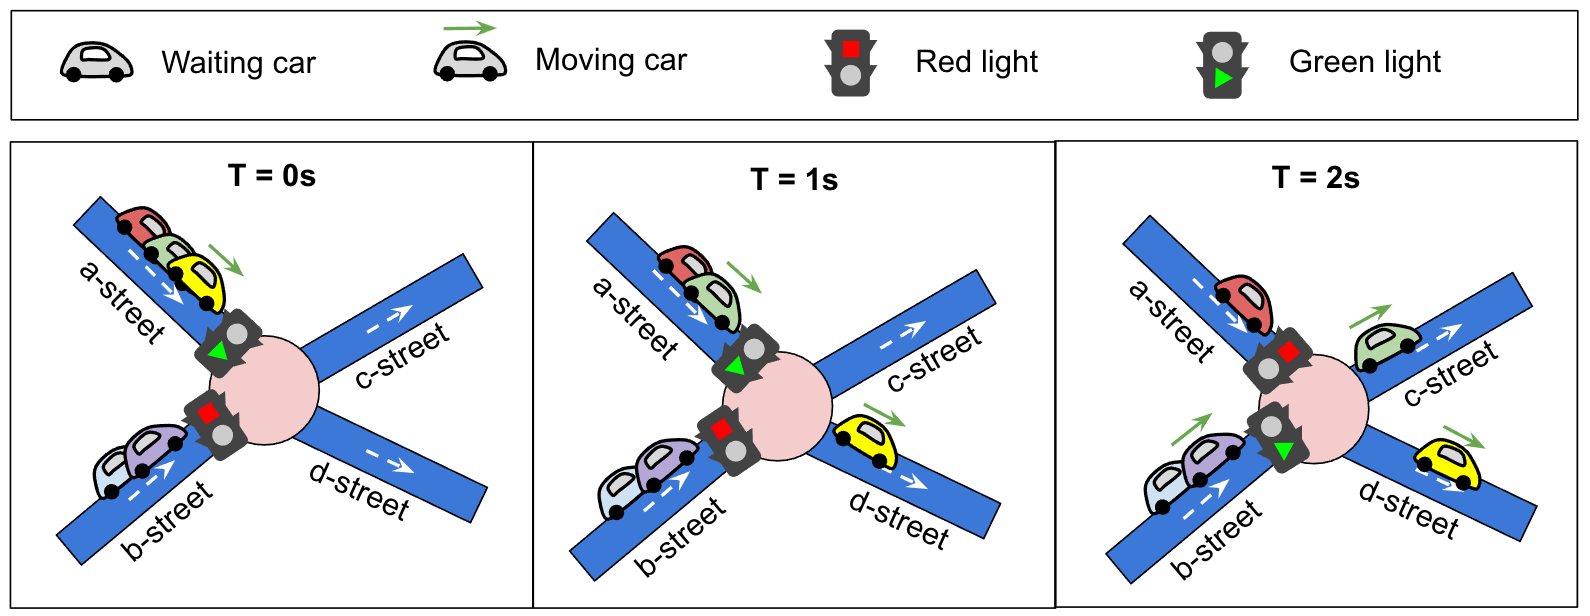
\includegraphics[width=1.0\linewidth]{img/figure2-abc.png}
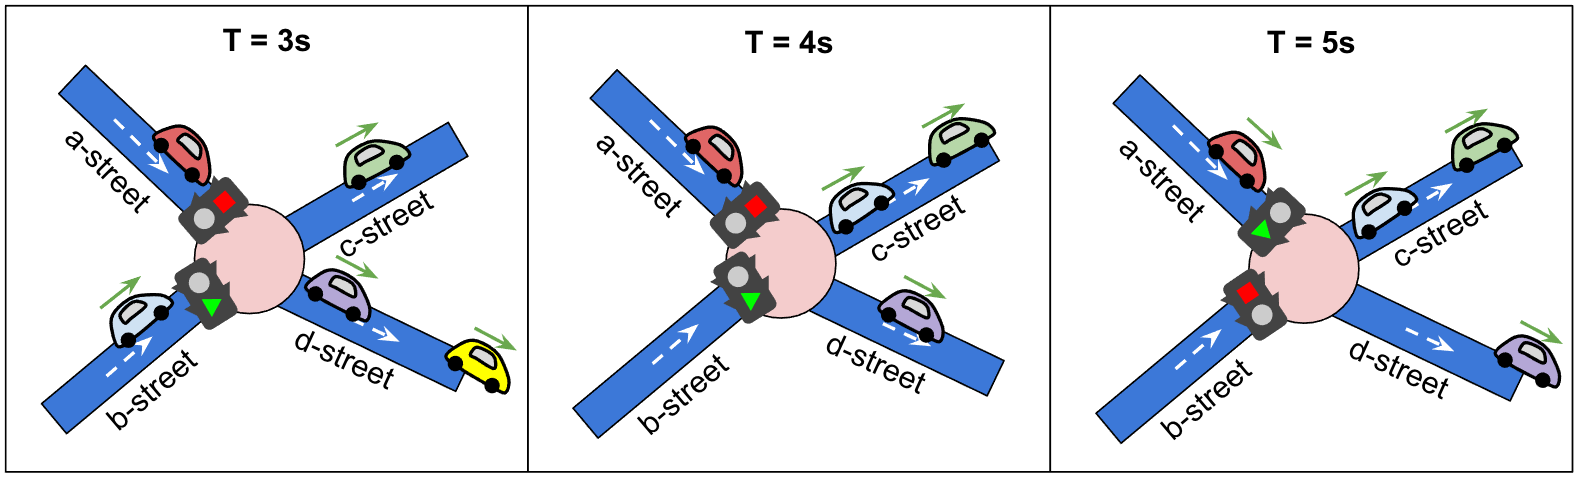
\includegraphics[width=1.0\linewidth]{img/figure2-def.png}
\small{Example of a schedule {[Google Hash Code 2021]}. \\
First, a-street has a green light for 2 seconds, then b-street for 3 seconds. \\
One car can pass each second.}
\end{center}
\end{posterbox}

%
% FOOTER
%
\begin{posterbox}[column=0, span=2, name=footer, below=something1,
	textborder=none, headerborder=none, boxheaderheight=0pt,
	boxColorOne=black!3]{}
\vspace{-1.5ex}
\qrcode[height=1.5cm]{https://github.com/davidruda/Traffic-Signal-Optimization} 
\hspace{0.5ex} \url{github.com/davidruda/Traffic-Signal-Optimization}
% \fancyqr[image=\scalebox{1.2}{\faGithub}, image padding=1,color=black!90!gray]{https://github.com/davidruda/Traffic-Signal-Optimization}
\end{posterbox}

%
% RIGHT COLUMN
%
% It is usually best to fill most of the poster with your results and
% conclusions. Again, use simple annotated pictures wherever possible. Plots
% with measurements are perfect, tables are also good.
%

\begin{posterbox}[column=1, name=something2, headerColorOne=yellow!80!orange!95!black, boxColorOne=yellow!33]
{Score}
The total score of the schedules $\bm{\theta}$ is defined as
\begin{equation*}
    SCORE(\bm{\theta}) = \sum_{c \in C}
	    \begin{cases}
        \mathrm{F} + (\mathrm{D} - t(c; \bm{\theta})), & \text{if $t(c; \bm{\theta}) \leq \mathrm{D}$}, \\
        0, & \text{otherwise},
    \end{cases}
\end{equation*}
i.e., cars arriving before or at the simulation end get the bonus plus extra points for arriving early; cars arriving later get zero. \\

$\mathrm{D}$ - simulation duration \\
$\mathrm{F}$ - fixed bonus for reaching the destination \\
$t(c; \bm{\theta})$ - arrival time of car $c$

\end{posterbox}

\begin{posterbox}[column=1, name=result1, below=something2]{Optimization Process}
\begin{minipage}{0.5\linewidth}
    \centering
    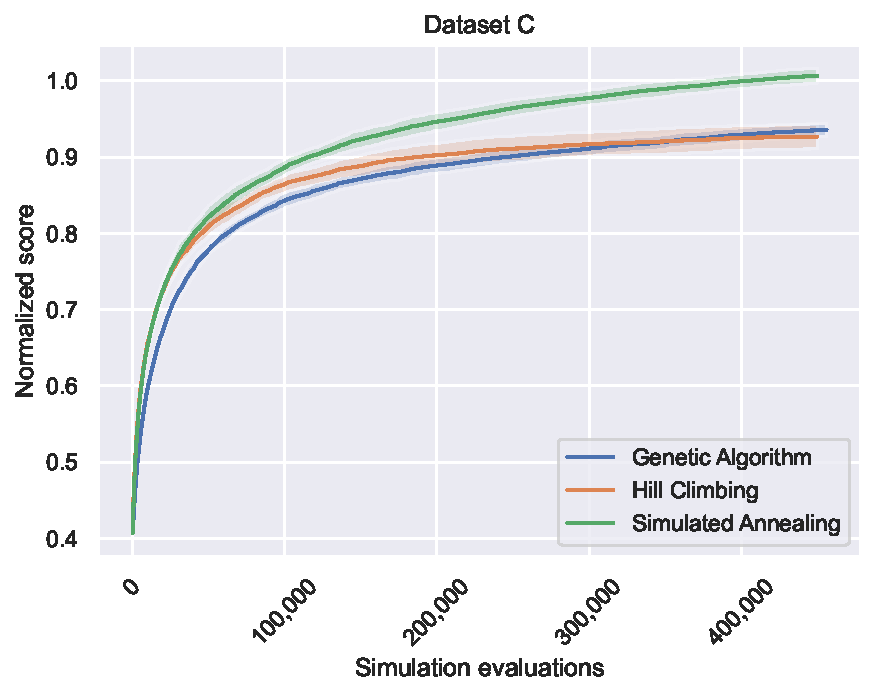
\includegraphics[width=1.\linewidth]{img/c_Genetic_Algorithm_Hill_Climbing_Simulated_Annealing.pdf}
    % \caption*{Caption for image 1}
\end{minipage}\hfill
\begin{minipage}{0.5\linewidth}
    \centering
    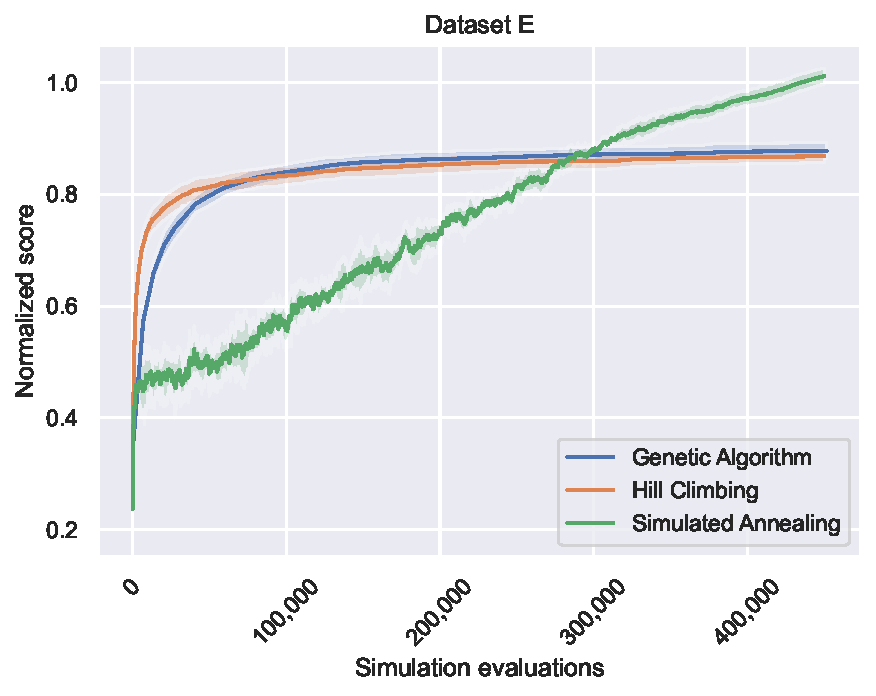
\includegraphics[width=1.\linewidth]{img/e_Genetic_Algorithm_Hill_Climbing_Simulated_Annealing.pdf}
    % \caption*{Caption for image 2}
\end{minipage}
\begin{center}
{\small Convergence of optimization algorithms on datasets C and E. \\
All algorithms have a fixed budget of simulation evaluations.}
\end{center}
\end{posterbox}

\begin{posterbox}[column=1, name=result2, below=result1]{Results}
\begin{center}

% AVERAGE SCORE OUT OF 10 SEEDS (NORMALIZED SCORE)
\begin{tabular}{lrrrr}
% \toprule
% Dataset & \textcolor{myblue}{\textbf{GA} (norm)} & \textcolor{myorange}{\textbf{HC} (norm)} & \textcolor{mygreen}{\textbf{SA} (norm)} \\
Dataset & \textbf{\# Params} & \textbf{\textcolor{myblue}{\shortstack{Genetic \\ Algorithm}}} & \textbf{\textcolor{myorange}{\shortstack{Hill \\ Climbing}}} & \textbf{\textcolor{mygreen}{\shortstack{Simulated \\ Annealing}}} \\
\midrule
\textbf{B} & 5,974 & 0.91 & 0.87 & \textbf{0.97} \\
\textbf{C} & 14,008 & 0.94 & 0.93 & \textbf{1.01\rlap{\textsuperscript{*}}} \\
\textbf{D} & 167,748 & 0.90 & \textbf{0.92} & 0.92 \\
\textbf{E} & 1,386 & 0.88 & 0.87 & \textbf{1.01\rlap{\textsuperscript{*}}} \\
\textbf{F} & 10,002 & 0.93 & 0.93 & \textbf{0.94} \\
\bottomrule
\end{tabular} \\
{\small The scores are averaged over 10 seeds and normalized: \\
0.00 - our baseline, 1.00 - maximum known score \\
\textit{\textbf{\textsuperscript{*}}New maximum known score}}

\end{center}
\end{posterbox}

\begin{posterbox}[column=1, name=result3, below=result2, headerColorOne=green!50!yellow, boxColorOne=green!10]{Main result}
\large\bfseries
\vspace{1ex}
\begin{center}
	\textcolor{mygreen}{Simulated Annealing} consistently outperforms the other methods, setting new maximum known scores on datasets C and E. \\
\end{center}
% \vspace{.25ex}
\end{posterbox}

\begin{posterbox}[column=1, name=conclusion, below=result3,
	% bottomaligned=something2
]{Conclusions}
\begin{itemize}
\item All three algorithms achieved good results across all datasets
\item Genetic Algorithm's broad search is less beneficial for this particular problem
\item Single-state methods like Simulated Annealing seem more suitable
\end{itemize}
\vspace{-1ex}
Possible future work:
\begin{itemize}
\item Compare methods under equal runtime budget, not only by equal simulation evaluations
\item Test other single-state methods (Tabu Search, Iterated Local Search)
% \item include long-term goals
\end{itemize}
\end{posterbox}

\end{poster}
\end{document}
